\documentclass{article}
\usepackage[english, russian]{babel}
\usepackage[T2A]{fontenc}
\usepackage[utf8]{inputenc}
%
\usepackage[russian]{babel}
\usepackage{graphicx}
%\graphicspath{{image constructors/}}
%\DeclareGraphicsExtensions{.png,.svg,.eps}
\usepackage[a4paper,left=2.5cm, right=1.5cm, top=2.5cm, bottom=2.5cm]{geometry}
\usepackage{amsfonts}
\usepackage{amsmath}
\usepackage{amssymb}
\usepackage{autonum}
%\usepackage{hyperref}

\newtheorem{deftext}{определение}
\newtheorem{theoremtext}{теорема}
\newtheorem{commenttext}{замечание}
\newtheorem{exampletext}{пример}

\begin{document}
	\large
	\section{модуль ontology.py}
	Здесь хранится классы для хранения и взаимодействия с онтологией
	
	\subsection{класс Ontology}
	этот класс хранит и обрабатывает онтологию.
	
	Ограничения на онтологию:
	\begin{itemize}
		\item все классы имеют различные названия
		\item все отношения исходящие из 1 класса имеют одинаковое название
		\item все сущности из одного класса имеют различные названия
		\item фиксированное отношение между фиксированными сущностями может существовать только в единственном виде(без множественности)
	\end{itemize}\ \\
	
	\begin{enumerate}
	\item def \_\_init\_\_(self, fileName=None)
		\begin{itemize}
			\item fileName - файл с сохраненной онтологией с папке ./saved/
		\end{itemize}
		конструктор, создающий пустую онтологию при fileName=None
	
	\item def addClass(self,className)
	\begin{itemize}
		\item className - название класса
	\end{itemize}
	добавление нового класса, с генерацией ошибки при существовании добавляемого класса
	
	\item def changeClass(self,oldClassName, newClassName)
	\begin{itemize}
		\item oldClassName - старое название класса
		\item newClassName - новое название класса
	\end{itemize}
	изменение названия класса, с генерацией ошибки при существовании нового класса или отсутствии старого класса
	
	\item def deleteClass(self,className,deep=False)
	\begin{itemize}
		\item className - название класса
		\item deep - метка для глубокого удаления
	\end{itemize}
	удаление класса, с генерацией ошибки при несуществовании класса, при глубоком удалении со всеми связями на него и из него и с генерацией ошибки при наличии связей
	
	\item def addRelationship(self, relationshipName, outClassName, inClassName)
	\begin{itemize}
		\item relationshipName - название отношения
		\item outClassName - название выходного класс
		\item inClassName - название входного класс
	\end{itemize}
	создание отношения, с генерацией ошибки при несуществовании одного из классов или уже существовании отношения
	
	\item def changeRelationship(self, oldRelationshipName, newRelationshipName, outClassName)
	\begin{itemize}
		\item oldRelationshipName - новое название отношения
		\item newRelationshipName - старое название отношения
		\item outClassName - название выходного класса
	\end{itemize}
	изменение названия отношения, с генерацией ошибки при несуществовании старого отношения или существования нового отношения или несуществовании выходного класса
	
	\item def deleteRelationship(self, relationshipName, outClassName, deep=False)
	\begin{itemize}
		\item relationshipName - название отношения
		\item outClassName - название выходного класса
		\item deep - метка дял глубокого удаления
	\end{itemize}
	удаление отношения с генерацией ошибки при несуществовании отношения или несуществовании выходного класса, с удалением свех связанных связей при глубоком удалении и генерацией ошибки при наличии связей при не глубоком удалении
	
	\item def addEntity(self, entityName, className)
	\begin{itemize}
		\item entityName - название сущности
		\item className - название класса
	\end{itemize}
	создание сущности класса, с генерацией ошибки при существовании сущности или несуществовании класса
	
	\item def changeEntity(self, oldEntityName, newEntityName, className)
	\begin{itemize}
		\item oldEntityName - название старой сущности
		\item newEntityName - название новой сущности
		\item className - название класса
	\end{itemize}
	изменение названия сущности класса, с генерацией ошибки при не существовании старой сущности или существовании новой сущности или не существовании класса
	
	\item def deleteEntity(self, entityName, className, deep=False)
	\begin{itemize}
		\item entityName - название сущности
		\item className - название класса
		\item deep - метка для глубокого удаления
	\end{itemize}
	удаление сущности класса, с генерацией ошибки при не существовании сущности или не существовании класса, с удалением всех связей при глубоком удалении и генерацией ошибки при наличии связей при не глубоком удалении
	
	\item def addEntityRelationship(self, relationshipName, outClassName, outEntityName, inEntityName)
	\begin{itemize}
		\item relationshipName - название отношения
		\item outClassName - название выходного класса
		\item outEntityName - название выходной сущности
		\item inEntityName - название входной сущности
	\end{itemize}
	добавление связи между сущностями, с генерацией ошибки при несуществовании отношения класса или не существовании выходного класса или выходной сущности или входной сущности или существования отношения между сущностями
	
	\item def deleteEntityRelationship(self, relationshipName, outClassName, outEntityName, inEntityName)
	\begin{itemize}
		\item relationshipName - название отношения
		\item outClassName - название выходного класса
		\item outEntityName - название выходной сущности
		\item inEntityName - название входной сущности
	\end{itemize}
	удаление связи между сущностями, с генерацией ошибки при несуществовании отношения класса или не существовании выходного класса или выходной сущности или входной сущности или не существования отношения между сущностями
	
	\item def getAllClasses(self)
	\begin{itemize}
		\item return - список с названиями классов
	\end{itemize}
	получение списка классов
	
	\item def getAllRelationshipsForOutClass(self, className)
	\begin{itemize}
		\item className - название класса
		\item return - список с названиями отношений
	\end{itemize}
	получение все отношений класса, с генерацией ошибки при не существовании класса
	
	\item def getAllEntitiesForClass(self, className)
	\begin{itemize}
		\item className - название класса
		\item return - список с названиями сущностей класса
	\end{itemize}
	получение всех сущностей класса, с генерацией ошибки при не существовании класса
	
	\item def getAllRelationshipedEntitiesForOutEntity(self, outEntityName, outClassName)
	\begin{itemize}
		\item outEntityName - название сущности класса
		\item outClassName - название выходного класса
		\item return - список кортеджей вида (название класса, название сущности класса, название отношения)
	\end{itemize}
	получение всех сущностей класса связанных с заданной сущностью, с генерацией ошибки при не существования заданной сущности класса или несуществовании выходного класса
	
	\item def getAllRelationshipedEntitiesForOutEntityForInClass(self, outEntityName, outClassName, inClassName)
	\begin{itemize}
		\item outEntityName - название сущности класса
		\item outClassName - название выходного класса
		\item inClassName - название входного класса
		\item return - список кортеджей вида (название класса, название сущности класса)
	\end{itemize}
	получение всех сущностей класса связанных с заданной сущностью из заданного входного класса, с генерацией ошибки при не существования заданной сущности класса или несуществовании выходного класса или не существовании входного класса
	
	\item getAllRelationshipedEntitiesForOutEntityForRelationship(self, outEntityName, outClassName, relationshipName)
	\begin{itemize}
		\item outEntityName - название сущности класса
		\item outClassName - название выходного класса
		\item relationshipName - название отношения
		\item return - список кортеджей вида (название класса, название сущности класса)
	\end{itemize}
	получение всех сущностей класса связанных с заданной сущностью заданным отношением, с генерацией ошибки при не существования заданной сущности класса или несуществовании выходного класса или не существовании отношения
	
	\item def saveToFile(self, fileName)
	\begin{itemize}
		\item fileName - название файла
	\end{itemize}
	сохранение онтологии в файл с папке /saved/
	
	\item def loadFromFile(self, fileName)
	\begin{itemize}
		\item fileName - название fileName
	\end{itemize}
	загрузка и обновление текущей онтологии из файла с папке /saved/
	
	\item def clear(self)
	отчистка онтологии (удаление всех данных)
	
	\end{enumerate}
	
	Пример использования на примере онтологии, изображенной на рисунке
	\begin{figure}[!h]
		\begin{center}
			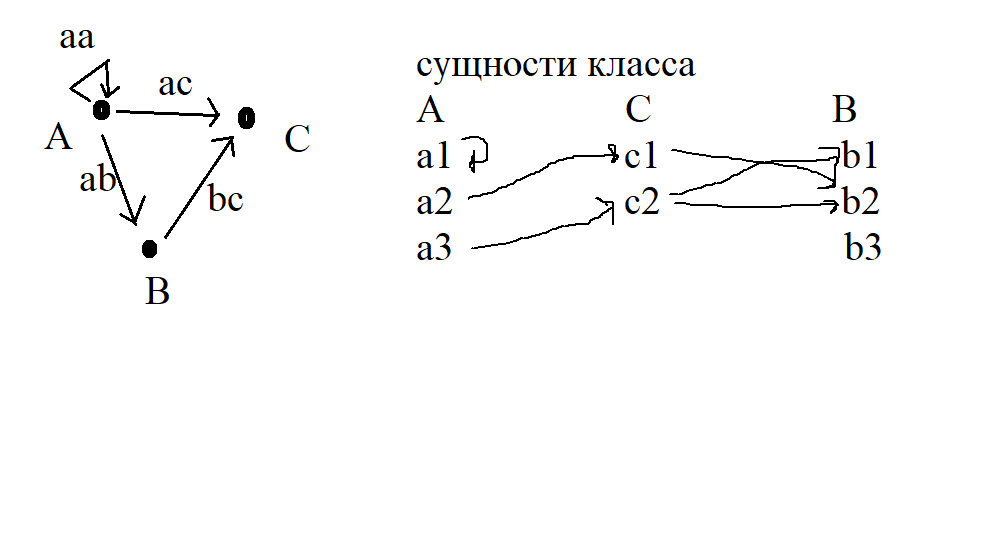
\includegraphics[scale=0.5]{example.png}
		\end{center}
	\end{figure}
	
	\normalsize
	\begin{verbatim}
	from ontology import *
	
	ont=Ontology()
	ont.addClass('A')
	ont.addClass('B')
	ont.addClass('CC')
	ont.addClass('D')
	ont.changeClass('CC','C')
	ont.deleteClass('D', True)
	print(ont.getAllClasses())# ['A', 'B', 'C']
	
	ont.addRelationship('aa','A','A')
	ont.addRelationship('ab','A','B')
	ont.addRelationship('ac','A','C')
	ont.addRelationship('cb_','C','B')
	ont.addRelationship('bb','B','B')
	ont.changeRelationship('cb_','cb','C')
	ont.deleteRelationship('bb','B', False)
	
	ont.addEntity('a1','A')
	ont.addEntity('a2','A')
	ont.addEntity('b1','B')
	ont.addEntity('b2','B')
	ont.addEntity('b3','B')
	ont.addEntity('c1','C')
	ont.addEntity('c2_','C')
	ont.addEntity('c3','C')
	ont.changeEntity('c2_','c2','C')
	ont.deleteEntity('c3','C')
	
	ont.addEntityRelationship('aa','A','a1','a1')
	ont.addEntityRelationship('ac','A','a2','c1')
	ont.addEntityRelationship('ac','A','a2','c2')
	ont.addEntityRelationship('cb','C','c1','b2')
	ont.addEntityRelationship('cb','C','c2','b2')
	ont.addEntityRelationship('cb','C','c2','b1')
	ont.addEntityRelationship('cb','C','c2','b3')
	ont.deleteEntityRelationship('cb','C','c2','b3')
	
	print(ont.getAllClasses())# ['A', 'B', 'C']
	print(ont.getAllRelationshipsForOutClass('A'))# ['aa', 'ab', 'ac']
	print(ont.getAllRelationshipsForOutClass('B'))# []
	print(ont.getAllRelationshipsForOutClass('C'))# ['cb']
	print(ont.getAllRelationshipsForOutClassToInClass('A','B'))# ['ab']
	print(ont.getAllRelationshipsForOutClassToInClass('A','A'))# ['aa']
	print(ont.getAllRelationshipsForOutClassToInClass('C','A'))# []
	print(ont.getAllEntitiesForClass('A'))# ['a1', 'a2']
	print(ont.getAllEntitiesForClass('B'))# ['b1', 'b2', 'b3']
	print(ont.getAllEntitiesForClass('C'))# ['c1', 'c2']
	print(ont.getAllRelationshipedEntitiesForOutEntity('a1','A'))# [('A', 'a1', 'aa')]
	print(ont.getAllRelationshipedEntitiesForOutEntity('a2','A'))
	# [('C', 'c1', 'ac'), ('C', 'c2', 'ac')]
	print(ont.getAllRelationshipedEntitiesForOutEntity('b1','B'))# []
	print(ont.getAllRelationshipedEntitiesForOutEntityForInClass('a2','A','C'))
	# [('c1', 'ac'), ('c2', 'ac')]
	print(ont.getAllRelationshipedEntitiesForOutEntityForInClass('a2','A','B'))# []
	print(ont.getAllRelationshipedEntitiesForOutEntityForRelationship('a2','A','ac'))# ['c1', 'c2']
	print(ont.getAllRelationshipedEntitiesForOutEntityForRelationship('a2','A','ab'))# []
	ont.saveToFile('ont1.txt')
	
	ont.loadFromFile('ont1.txt')
	#...
	ont.crear()
	ont=Ontology('ont1.txt')
	#...
	\end{verbatim}
	\large
	
	\section{модуль ontologyStatistics.py}
	Здесь хранится классы для хранения и взаимодействия с онтологией
	
	\subsection{класс SimpleStatistics}
	этот класс состоит только из статических методов и вычисляет простые соотношения и количества для сущностей класса и их связей.
	\ \\
	
	\begin{enumerate}
		\item def getCountEntitiesForClass(ontology, className)
		\begin{itemize}
			\item ontology - объект ontology.Ontology
			\item className - название класса
			\item return - целочисленное число
		\end{itemize}
		количество сущностей класса, с генерацией ошибки при не существовании добавляемого класса
		
		\item def getMaxCountEntitiesForAnyClass(ontology)
		\begin{itemize}
			\item ontology - объект ontology.Ontology
			\item return - целочисленное число
		\end{itemize}
		максимальное количество сущностей класса для одного  класса
		
		\item def getEmptyClasses(ontology)
		\begin{itemize}
			\item ontology - объект ontology.Ontology
			\item return - список с названиями классов
		\end{itemize}
		список классов без сущностей
		
		\item def getCountEntitiesForClassWhitchSatisfyRelationships(ontology, className, withRelationships, withoutRelationships)
		\begin{itemize}
			\item ontology - объект ontology.Ontology
			\item className - название класса
			\item withRelationships - список с названиями присутствующих отношений
			\item withoutRelationships - список с названиями отсутствующих отношений
			\item return - целочисленное число
		\end{itemize}
		количество сущностей класса из заданного класса, у которых нет связей соответствующих отсутствующим отношениям и есть все связи хотя бы по одному разу соответствующие присутствующим отношениям, с генерацией исключения при несуществовании класса или несуществовании идного из указанных отношений
		
		\item def getEntitiesForClassWhitchSatisfyRelationships(ontology, className, withRelationships, withoutRelationships)
		\begin{itemize}
			\item ontology - объект ontology.Ontology
			\item className - название класса
			\item withRelationships - список с названиями присутствующих отношений
			\item withoutRelationships - список с названиями отсутствующих отношений
			\item return - список названий сущностей класса
		\end{itemize}
		список сущностей класса из заданного класса, у которых нет связей соответствующих отсутствующим отношениям и есть все связи хотя бы по одному разу соответствующие присутствующим отношениям, с генерацией исключения при несуществовании класса или несуществовании одного из указанных отношений
		
		\item def getAverageLinkBetweenClassesFor(ontology, outClassName, inClassName, forInClass = False)
		\begin{itemize}
			\item ontology - объект ontology.Ontology
			\item outClassName - название выходного класса
			\item inClassName - название входного класса
			\item forInClass - метка вычислений для входного класса(иначе дял выходного класса)
			\item return - вещественное число
		\end{itemize}
		среднее количество связей выходящий из сущностей класса выходного класса в сущности класса входного класса относительно количества сущностей класса для которого происходит вычисление, с генерацией исключения при несуществовании класса
		
		\item def getAverageLinkBetweenClassesWhitchSatisfyRelationships(ontology, outClassName, inClassName, withRelationships, withoutRelationships, forInClass = False)
		\begin{itemize}
			\item ontology - объект ontology.Ontology
			\item outClassName - название выходного класса
			\item inClassName - название входного класса
			\item withRelationships - список с названиями присутствующих отношений
			\item withoutRelationships - список с названиями отсутствующих отношений
			\item forInClass - метка вычислений для входного класса(иначе дял выходного класса)
			\item return - вещественное число
		\end{itemize}
		среднее количество связей выходящий из сущностей класса выходного класса в сущности класса входного класса относительно количества сущностей класса для которого происходит вычисление, где учитываются только сущности класса у которых не существует связей соответствующих отсутствующим отношениям и существуют связи соответствующие всем присутствующим отношениям, с генерацией исключения при несуществовании класса или несуществовании одного из указанных отношений 
		
		\item def getAverageLinkBetweenClassesForSpecifiedRelationships(ontology, outClassName, inClassName, specifiedRelationships, forInClass = False)
		\begin{itemize}
			\item ontology - объект ontology.Ontology
			\item outClassName - название выходного класса
			\item inClassName - название входного класса
			\item specifiedRelationships - список с названиями подсчитывающихся отношений
			\item forInClass - метка вычислений для входного класса(иначе дял выходного класса)
			\item return - вещественное число
		\end{itemize}
		среднее количество связей, соответствующих подсчитывающимся отношениям, выходящий из сущностей класса выходного класса в сущности класса входного класса относительно количества сущностей класса для которого происходит вычисление, с генерацией исключения при несуществовании класса или несуществовании одного из указанных отношений 
		
		\item def getAverageLinkBetweenClassesForSpecifiedRelationshipsWhitchSatisfyRelationships(
		ontology, outClassName, inClassName, specifiedRelationships, withRelationships, withoutRelationships, forInClass = False)
		\begin{itemize}
			\item ontology - объект ontology.Ontology
			\item outClassName - название выходного класса
			\item inClassName - название входного класса
			\item specifiedRelationships - список с названиями подсчитывающихся отношений
			\item withRelationships - список с названиями присутствующих отношений
			\item withoutRelationships - список с названиями отсутствующих отношений
			\item forInClass - метка вычислений для входного класса(иначе дял выходного класса)
			\item return - вещественное число
		\end{itemize}
		среднее количество связей, соответствующих подсчитывающимся отношениям, выходящий из сущностей класса выходного класса в сущности класса входного класса относительно количества сущностей класса для которого происходит вычисление, где учитываются только сущности класса у которых не существует связей соответствующих отсутствующим отношениям и существуют связи соответствующие всем присутствующим отношениям, с генерацией исключения при несуществовании класса или несуществовании одного из указанных отношений 
	\end{enumerate}
	
	Пример использования
	
	\normalsize
	\begin{verbatim}
		from ontology import *
		from ontologyStatistics import *
		
		ont=Ontology()
		ont.addClass('A')
		ont.addClass('B')
		ont.addClass('C')
		ont.addClass('D')
		ont.addRelationship('ab1','A','B')
		ont.addRelationship('ab2','A','B')
		ont.addRelationship('ac1','A','C')
		ont.addRelationship('ac2','A','C')
		ont.addEntity('a1','A')
		ont.addEntity('a2','A')
		ont.addEntity('a3','A')
		ont.addEntity('a4','A')
		ont.addEntity('a5','A')
		ont.addEntity('a6','A')
		ont.addEntity('a7','A')
		ont.addEntity('a8','A')
		ont.addEntity('a9','A')
		ont.addEntity('a10','A')
		ont.addEntity('b1','B')
		ont.addEntity('b2','B')
		ont.addEntity('b3','B')
		ont.addEntity('c1','C')
		ont.addEntityRelationship('ac1','A','a1','c1')
		ont.addEntityRelationship('ac1','A','a2','c1')
		ont.addEntityRelationship('ac1','A','a3','c1')
		ont.addEntityRelationship('ac1','A','a4','c1')
		ont.addEntityRelationship('ac2','A','a4','c1')
		ont.addEntityRelationship('ab1','A','a1','b1')
		ont.addEntityRelationship('ab2','A','a1','b1')
		ont.addEntityRelationship('ab1','A','a1','b2')
		ont.addEntityRelationship('ab2','A','a2','b2')
		ont.addEntityRelationship('ab1','A','a3','b2')
		ont.addEntityRelationship('ab1','A','a3','b3')
		ont.addEntityRelationship('ab1','A','a4','b3')
		ont.addEntityRelationship('ab2','A','a4','b3')
		ont.addEntityRelationship('ab1','A','a5','b3')
		
		print(SimpleStatistics.getCountEntitiesForClass(ont,'A'))#10
		print(SimpleStatistics.getCountEntitiesForClass(ont,'B'))#3
		print(SimpleStatistics.getCountEntitiesForClass(ont,'D'))#0
		print(SimpleStatistics.getMaxCountEntitiesForAnyClass(ont))#10
		print(SimpleStatistics.getEmptyClasses(ont))#['D']
		print(SimpleStatistics.getEntitiesForClassWhitchSatisfyRelationships(
		    ont, 'A', set(['ac1','ab1']), set(['ac2'])))#['a1','a3']
		print(SimpleStatistics.getCountEntitiesForClassWhitchSatisfyRelationships(
		    ont, 'A',set(['ac1','ab1']), set(['ac2'])))#2
		print(SimpleStatistics.getCountEntitiesForClassWhitchSatisfyRelationships(
		    ont, 'A',set(), set(['ac2'])))#9
		print(SimpleStatistics.getAverageLinkBetweenClassesFor(
		    ont, 'A', 'B', True))#3.0
		print(SimpleStatistics.getAverageLinkBetweenClassesFor(
		    ont, 'A', 'B', False))#0.9
		print(SimpleStatistics.getAverageLinkBetweenClassesWhitchSatisfyRelationships(
		    ont, 'A', 'B', set(['ac1']), set(['ac2']), True))#2.0
		print(SimpleStatistics.getAverageLinkBetweenClassesWhitchSatisfyRelationships(
		    ont, 'A', 'B', set(['ac1']), set(['ac2']), False))#0.6
		print(SimpleStatistics.getAverageLinkBetweenClassesForSpecifiedRelationships(
		    ont, 'A', 'B', set(['ab1']), True))#2.0
		print(SimpleStatistics.getAverageLinkBetweenClassesForSpecifiedRelationships(
		    ont, 'A', 'B', set(['ab1']), False))#0.6
		print(SimpleStatistics.getAverageLinkBetweenClassesForSpecifiedRelationships(
		    ont, 'A', 'B', set(['ab1','ab2']), True))#3.0
		print(SimpleStatistics.getAverageLinkBetweenClassesForSpecifiedRelationships(
		    ont, 'A', 'B', set(['ab1','ab2']), False))#0.9
		print(SimpleStatistics.
		    getAverageLinkBetweenClassesForSpecifiedRelationshipsWhitchSatisfyRelationships(
		    ont, 'A', 'B', set(['ab1']), set(['ac1']), set(['ac2']), True))#1.3333333333333
		print(SimpleStatistics.
		    getAverageLinkBetweenClassesForSpecifiedRelationshipsWhitchSatisfyRelationships(
		    ont, 'A', 'B', set(['ab1']), set(['ac1']), set(['ac2']), False))#0.4
	\end{verbatim}
	\large
\end{document}